\documentclass[a4paper,titlepage]{article}

\usepackage[T1]{fontenc}
\usepackage[utf8]{inputenc}
\usepackage[italian]{babel}
\usepackage{url}
\usepackage{verbatim}
\usepackage{titlepic}
\usepackage{graphicx}
%\usepackage{syntonly}
%\syntaxonly

\pagestyle{headings}

%\includeonly{}


\begin{document}

\titlepic{\includegraphics[width=4cm]{images/unirm2.png}}

\title{
  Il worm Code Red
}
\author{
  Simone Bassani\\
  \texttt{sbassani92@gmail.com}
  \and
  Simone Falvo\\
  \texttt{smvfal@gmail.com}
}

\date{}


\maketitle

%\input{sections/abstract}

\tableofcontents
\newpage

\section{Introduzione}
A luglio del 2001 più di 359.000 computer sono stati infettati, in meno di 14 ore, da un worm chiamato “Code Red”.\\
Per infettare un dispositivo Code Red sfruttava una vulnerabilità dei server IIS di Microsoft, e la vulnerabilità riguardava l’overflow di un buffer usato nella ricezione delle richieste per il server. I dispositivi infettati venivano poi utilizzati per effettuare un attacco DDoS ai danni della Casa Bianca.\\
E’ stato scoperto il 13 luglio 2001 da Marc Maiffret e Myan Parmah, dipendenti di eEye Digital Security ed è diventato famoso come il malware più costoso del 2001.\\
Lo scopo di questo documento è di trattare l'incidente in maniera approfondita, partendo dalla descrizione dettagliata del comportamento del worm e dalla vulnerabilità sfruttata, per poi analizzare l'impatto che ha avuto sulla rete globale, quali sono stati i fattori che hanno permesso di provocare tanti danni e quali sono state le contromisure intraprese nel tentativo di porre fine alla sua diffusione. Infine abbiamo provato ad immaginare cosa sarebbe successo se il worm avesse agito in maniera indisturbata, e quali alternative si sarebbero potute adottare per limitare i danni in maniera più efficace.\\


\section{Dettagli incidente}
\subsection{Timeline}
Questa timeline contiene i passi più importanti della diffusione del worm, e bisogna notare la presenza di due diverse versioni di Code Red che sono state rilasciate in quel periodo:
\begin{itemize}
\item[-]18 giugno: eEye Security rende nota pubblicamente la vulnerabilità dei web server IIS;
\item[-]26 giugno: Microsoft rilascia una patch per risolvere la vulnerabilità;
\item[-]12 luglio: una prima versione del worm “Code Red” viene rilasciata, residente in memoria, seme statico, scanning randomico;
\item[-]19 luglio: il worm “CodeRed v2” viene rilasciato con seme dinamico.
\end{itemize}
%%%%%%%%%%%%%%%%%%%%%%%%%%%%%%%%%%%%%%%%%%%%%%%%%%%%%%%%%%%%%%%%%%%%%%%%%%%%%%%%%%%%%%%%%%%%%%%
\subsection{Caratteristiche e comportamento}
Il payload dei pacchetti provenienti dal worm si presenta nel seguente modo (figura~\ref{payload}):
\begin{figure}[!h]
\centering

\includegraphics[width=0.8\textwidth]{images/payload.eps}
\caption{payload}
\label{payload}
\end{figure}
La serie di “N” con cui inizia il payload serve esclusivamente per generare l’overflow del buffer, mentre l’istruzione vera e propria, inserita dall’attaccante, è la parte seguente. A causa dell’overflow l’host interpreta le stringhe come istruzioni, le esegue portando all’esecuzione del comando arbitrario inserito dall’attaccante.

La caratteristica del worm Code Red è il suo comportamento dinamico, dipendente dal giorno del mese. Lo schema utilizzato è il seguente:
\begin{itemize}
\item[-]Giorni 1-19 : il worm prova a diffondersi cercando altri server IIS nella rete Internet;
\item[-]Giorni 20-27 : sfrutta le macchine che è riuscito ad infettare per lanciare un attacco DDoS contro diversi indirizzi IP (incluso quello della Casa Bianca 198.137.240.91);
\item[-]Giorni 28-fine del mese: va in “sleep”.
\end{itemize}
%%%%%%%%%%%%%%%%%%%%%%%%%%%%%%%%%%%%%%%%%%%%%%%%%%%%%%%%%%%%%%%%%%%%%%%%%%%%%%%%%%%%%%%%%%%%%%%
\subsection{Diffusione}
La diffusione è un aspetto critico per il worm Code Red. Lo schema seguito è il seguente:\\
\begin{enumerate}
\item Setup dell’ambiente iniziale del worm nel sistema infetto
\item Vengono creati 100 thread:
\begin{itemize}
\item[-]i primi 99 vengono usati per diffondere il worm attraverso la creazione di indirizzi IP randomici.
\item[-]il 100-esimo controlla la versione del sistema operativo (Windows NT/2000) del sistema in cui è in esecuzione:
i. se il sistema operativo è di lingua Inglese(US), la pagina web del web server viene cambiata figura~\ref{hacked}, e tale modifica resta attiva per 10 ore prima di sparire
ii. in caso contrario il 100-esimo thread si unisce agli altri 99 per diffondere il worm
\end{itemize}
\item Ogni thread controlla la presenza del file c:$\backslash$notworm
\begin{itemize}
\item[-]se il file è trovato, il worm va in sleep
\item[-]altrimenti i thread continuano nel processo di infezione di altri sistemi
\end{itemize}
\item Ogni thread controlla l’ora del sistema 
\end{enumerate}
Entrambe le versioni rilasciate del worm hanno utilizzato lo stesso schema, con la sola differenza del seme usato per generare indirizzi casuali, che è statico nella prima versione e dinamico nella seconda. Questo dettaglio è di fondamentale importanza, ed è stato il cambiamento vincente della seconda versione per ottenere una rapida diffusione su scala mondiale.\\
\begin{figure}[!h]
\centering
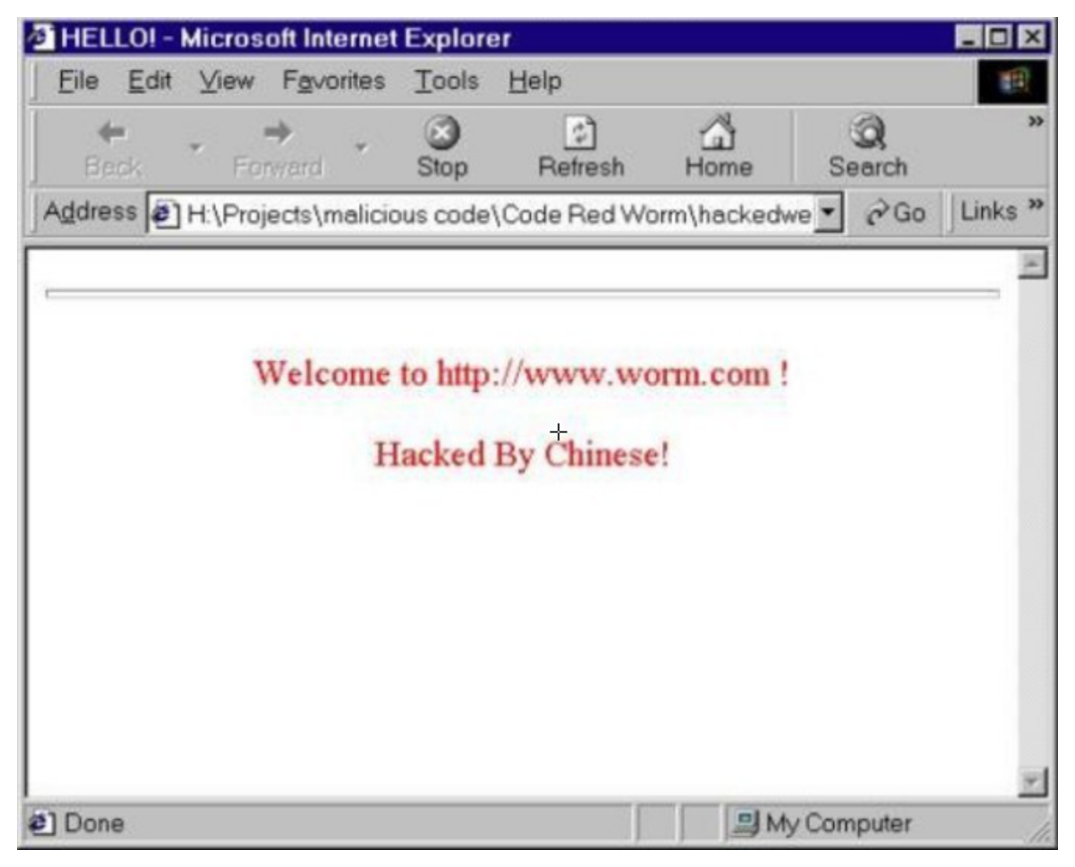
\includegraphics[width=0.7\textwidth]{images/hacked.eps}
\caption{defacing della pagina web}
\label{hacked}
\end{figure}
\subsection{Vulnerabilità}
La vulnerabilità è rappresentata da un buffer senza controllo sulla dimensione relativa alle richieste in arrivo, ed è presente in alcune estensioni ISAPI\footnote{L’ISAPI (Internet Services Application Programming Interface) è una tecnologia che permette agli sviluppatori di estendere le funzionalità fornite dal server IIS.} associate a “Microsoft Index Server” e “Indexing Service”\footnote{Microsoft Index Server e Indexing Service sono motori di ricerca e di indicizzazione. Permettono agli utenti di ricercare dati nei siti web o nei server web inserendo parole chiave, frasi o proprietà nei web browser.}. Il primo appartiene a “Windows NT 4.0 Option Pack” mentre il secondo è un servizio nativo di “Windows 2000”.\\
Un host che esegue una delle due può subire l’esecuzione di codice arbitrario a causa di tale vulnerabilità nell’estensione ISAPI idq.dll\footnote{Un estensione ISAPI è una dynamic link library (.dll) che usa ISAPI per fornire un set di funzioni web al di sopra di quelle fornite nativamente da IIS.\\
Idq.dll fornisce supporto per i file .ida-Internet Data Administration and .idq Internet Data Query.}. Questi processi sono eseguiti nel Local System context, permettendo all’attaccante di eseguire codice con privilegi Local System. Lo sfruttamento di questa vulnerabilità porta l’host target ad essere completamente compromesso in quanto l’attaccante potenzialmente può: eseguire codice arbitrario nel server, cambiare i contenuti contenuti in esso e riconfigurarlo.\\
Non serve che Index Server e Indexing Service siano in esecuzione per sfruttare la vulnerabilità, perché idq.dll è installato di default quando viene installato Microsoft IIS-Internet Information Server, quindi basta l’esecuzione di quest’ultimo.\\
%%%%%%%%%%%%%%%%%%%%%%%%%%%%%%%%
\subsubsection{Dettagli tecnici}
Nel suo processo di installazione, l’IIS installa diverse estensioni ISAPI, tra cui le “.dll” che forniscono funzionalità aggiuntive.
Quando un utente deve usare una funzione dell’estensione ISAPI manda una richiesta al server, anche se a volte è possibile chiamare l’estensione ISAPI direttamente. La richiesta dell’utente viene analizzata e IIS determina l’estensione ISAPI da usare, consultando una tabella con i mapping tra le estensioni dei file e ogni estensione ISAPI sul server.\\
L’estensione ISAPI che contiene la vulnerabilità è idq.dll, la quale fornisce due funzioni:
\begin{itemize}
\item[-]fornisce supporto per i file .ida (Internet Data Administration), che sono script che possono essere usati per gestire l’Indexing Service;
\item[-]processa i file .idq (Internet Data Query), usata per implementare ricerche custom.
\end{itemize}

Per sfruttare la vulnerabilità deve esistere un mapping tra i file .idq e .ida con l’ idq.dll.\\
Un attaccante che può stabilire una connessione con un server su cui è installato l’idq.dll, può condurre un attacco sfruttando tale vulnerabilità, riuscendo ad eseguire codice arbitrario sul server.\\
C’è un buffer non controllato nella parte di codice che gestisce le richieste in arrivo. L’arrivo di una richiesta “malformata” causerà un risultato diverso in base al tipo di contenuto della richiesta stessa:
\begin{itemize}
\item[-]dati randomici causeranno il fallimento del server. Nel caso di IIS 4.0 servirà l’intervento dell’amministratore, altrimenti nel caso di IIS 5.0 il server web sarà in grado di ripristinarsi in modo autonomo;
\item[-]codice eseguibile arbitrario causerà la sua esecuzione nel server web.
\end{itemize}

L’attaccante ottiene pieno controllo del server web, può eseguire ogni azione che desidera perché l’idq.dll è eseguito nel System Context.\\

A causa dei seri rischi legati a tale vulnerabilità, Microsoft ha consigliato agli utenti potenzialmente interessati da essa di prendere tempestive azioni di protezione. E’ stata rilasciata una patch per eliminare la vulnerabilità, mentre per i clienti impossibilitati ad installarla si poteva ricorrere alla rimozione dei mapping con i file .idq e .ida attraverso l’Internet Services Manager in IIS. Quest’ultima soluzione tuttavia non è da considerarsi come definitiva, in quanto a seguito di aggiunta/rimozioni di componenti addizionali di sistema poteva avvenire il reinserimento automatico dei mapping dannosi.\\

Chi può sfruttare la vulnerabilità? Attraverso essa può avere controllo sulla rete intera?\\
L’attaccante deve essere solo in grado di imporre una richiesta all’idq.dll . La presenza del mapping che associa i file .idq e .ida ad idq.dll, permette all’attaccante di stabilire una sessione web con il server, attraverso cui sfruttare la vulnerabilità.
Ci sono delle “best-practice” che aiutano a limitare la portata dell’intromissione di un attaccante. I web server, soprattutto quelli pubblici, sono sempre stati tra i target preferiti degli attacchi a causa della loro esposizione nella rete. Bisogna tenerne conto nel design della rete, e il primo obiettivo dev'essere quello di limitare le possibili conseguenze della compromissione di un server web.\\
In particolare si seguono due pratiche:
\begin{itemize}
\item[-]Isolare i web server nelle DMZ\footnote{una DMZ (DeMilitarized Zone) è una sottorete isolata, fisica o logica, la quale contiene dei server con lo scopo di renderli accessibili senza compromettere la sicurezza della rete.}, separandoli quindi dal resto della rete;\\
\item[-]Configurarli come macchine “stand-alone”. Se necessariamente devono far parte di un dominio, questo deve contenere solo macchine della DMZ. I web server non dovrebbero mai far parte dei più grandi domini nella rete.\\
\end{itemize}
Queste pratiche negano all’attaccante di arrivare facilmente al server, ma in caso di attacco riuscito questo potrebbe usare il server “conquistato” per attaccare altre macchine.\\
%%%%%%%%%%%%%%%%%%%%%%%%%%%%%%%%
\subsubsection{Fattori mitiganti}
\begin{itemize}
\item[-]La vulnerabilità può essere sfruttata solo se viene stabilita una sessione web con un server infetto. Per essere a rischio bisogna avere IIS, e questo è il caso di Windows 2000 Professional;
\item[-]La vulnerabilità non può essere sfruttata se non sono presenti i mapping con i .ida e .idq . Tali mapping possono essere rimossi come detto in precedenza;
\item[-]L’abilità di un attaccante che ha compromesso un web server è legata fortemente dall’architettura di rete. La “best practice” per l’architettura di rete riguardo le macchine da proteggere come i web server, prevede di minimizzarne l’esposizione verso un ambiente non controllato come Internet, posizionandole in DMZ, isolandole il più possibile dal resto della rete. Questa pratica può limitare pesantemente il raggio di azione di un attaccante.
\end{itemize}


\section{Responsabili}
In generale non è facile trovare il responsabile di un malware di tipo worm, dato che questo non legandosi a file nei dispositivi che infetta, non lascia una “scia” dietro di sé da sfruttare per risalire al primo dispositivo infetto, il “paziente zero”, ed eventualmente al suo creatore.\\
Anche per il caso di Code Red è stato possibile solo fare delle ipotesi, e la prima è stata fatta proprio dalla eEye.
La eEye ha sostenuto che il worm è stato creato a Makati City, Filippine, analogamente al worm “ILOVEYOU”.\\ 
Keith Rhodes, capo tecnico del General Accounting Office ha invece rilasciato un report in cui ha ipotizzato che Code Red è stato sviluppato presso l’Università Foshan in Guandong, Cina.\\
La Cina è stata uno dei primi paesi sospettati per lo sviluppo di Code Red, a causa del messaggio che veniva visualizzato dai dispositivi infettati all’accesso sulla rete (n.d.r. “Hacked by Chinese. Welcome to http://www.worm.com.”). Inoltre il lancio del virus è avvenuto poco dopo un incidente aereo che ha coinvolto un aereo spia militare americano e un jet da combattimento cinese.
Il personale dell’Università Foshan dichiarò però che, al lancio del worm, i laboratori si trovavano in ristrutturazione e l’Università era nel periodo di vacanza, facendo quindi perdere di credibilità questa possibile soluzione.\\
A favore di questa tesi ci furono delle rilevazioni eseguite da Dshield.org, le quali dimostrarono che il virus colpì prima gli Stati Uniti e altri Paesi prima di arrivare in Cina. Dunque l’origine di Code Red andrebbe cercata altrove.\\
Den Eichman, ingegnere capo della sicurezza per il CAS, sottolineò che l’infezione poteva essere partita anche da remoto, rendendo di fatto impossibile definire con sicurezza da dove fosse partito il worm.\\
Johannes Ullrich, operatore di Dshield.org ipotizzò invece che il worm fu lanciato da uno dei partecipanti al DefCon, convention annuale di hacker che si svolse a Las Vegas il 13 luglio.\\


\section{Diffusione e sistemi coinvolti}
Non esistono molti dati riguardo la diffusione e l’impatto di Code Red, ma sicuramente l’analisi svolta da Moore et al.~\cite{caida} è la più completa e significativa che è stata effettuata.\\
La loro analisi si è svolta analizzando due set di dati relativi al monitoraggio di pacchetti TCP SYN indesiderati che giungevano rispettivamente nella rete /8 di ricerca dell’università della California a San Diego e in altre due reti /16  del Lawrence Berkeley Laboratory.\\
Analizzando gli indirizzi IP di provenienza sono riusciti a determinare l’estensione della diffusione del worm e contando il numero di diversi indirizzi IP che effettuavano le scansioni ripetute è stato possibile effettuare una stima sul numero di host infettati.\\
I risultati hanno mostrato che tra la mezzanotte del 19 Luglio a quella del 20 Luglio sono stati infettati intorno ai 359000 distinti indirizzi IP provenienti da ogni parte del mondo, la figura ~\ref{spread} mostra la distribuzione geografica delle macchine infette. Inoltre poiché i dati raccolti costituiscono soltanto un campione delle richieste di connessione, il numero di host rilevati fornisce un lower bound per il numero totale di host compromessi.\\
\begin{figure}[!hbp]
\centering
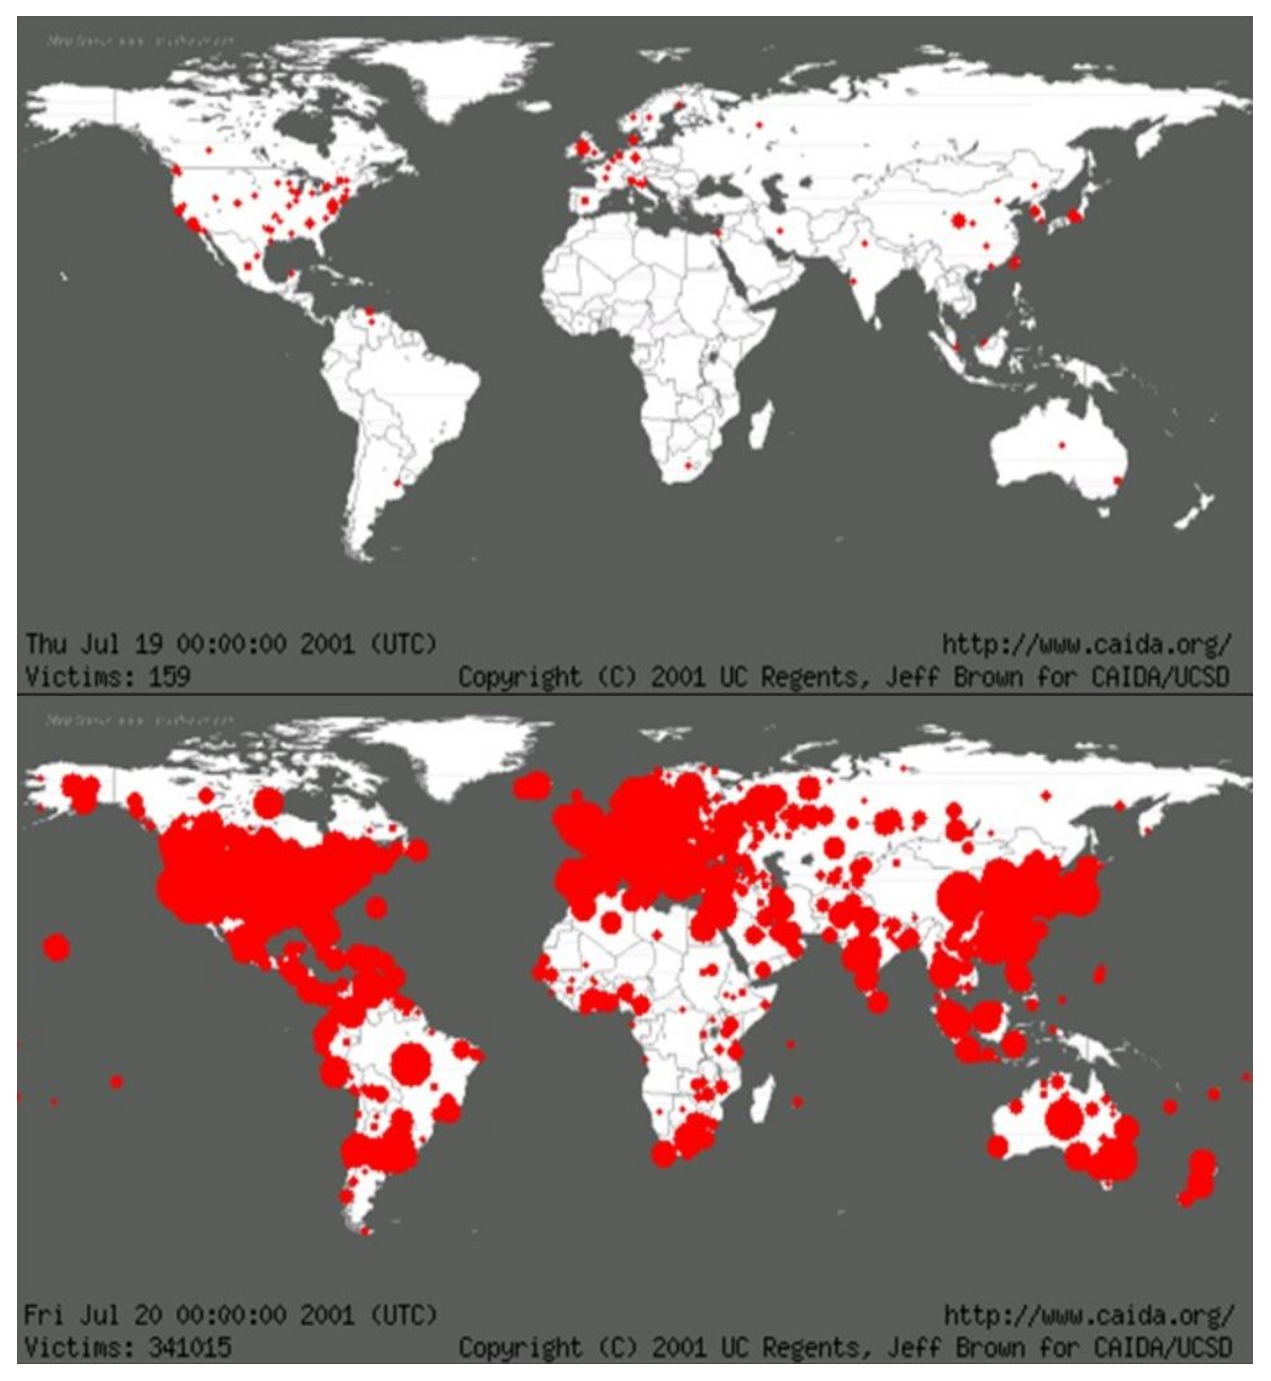
\includegraphics[width=0.8\textwidth]{images/spread.eps}
\caption{diffusione Code Red}
\label{spread}
\end{figure}
Le figure~\ref{infected} e~\ref{rate} danno un’idea del forte impatto che ha avuto la versione di Code Red a seme dinamico, infatti si vede che a partire dalla mattina del 19 Luglio c’è stato un improvviso incremento del tasso di infezione che ha raggiunto un valore di 2000 host al minuto. È interessante notare anche la decrescita esponenziale di tale tasso, dovuta probabilmente al conseguente stato di indisponibilità dei server, all’adozione di contromisure e ai gravi problemi causati alla rete globale che hanno portato ad un inevitabile rallentamento del traffico.\\
\begin{figure}
    \centering
    \begin{minipage}{0.5\textwidth}
        \centering
        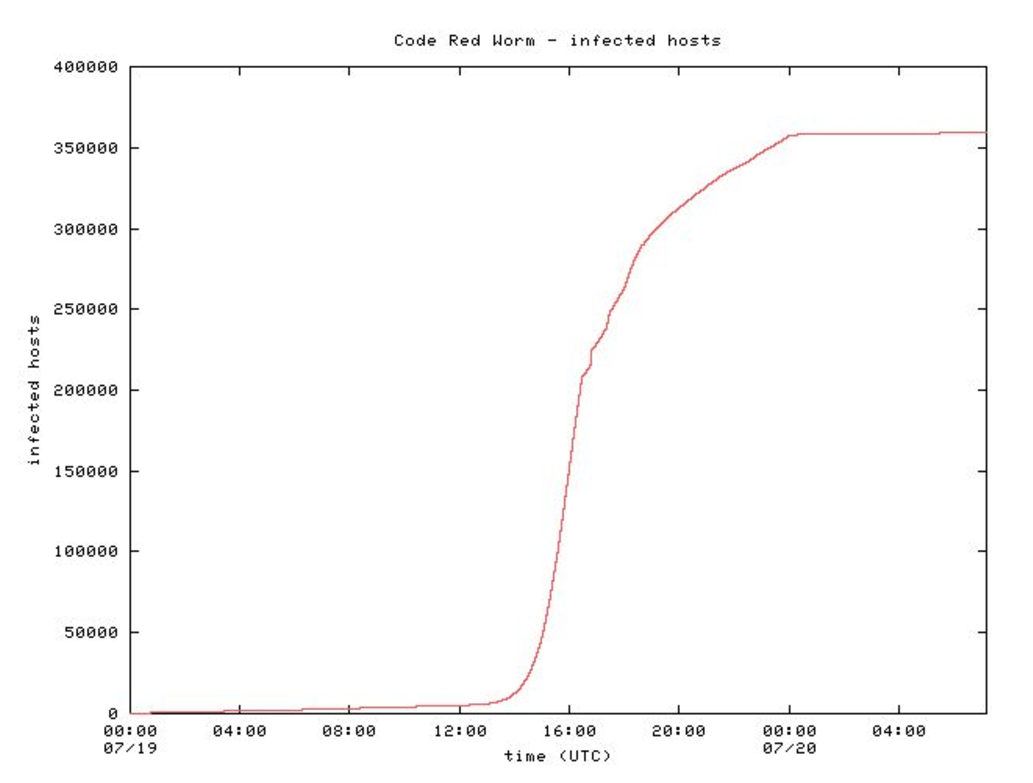
\includegraphics[width=0.95\textwidth]{images/infected} % first figure itself
        \caption{totale host infettati}
        \label{infected}
    \end{minipage}\hfill
    \begin{minipage}{0.5\textwidth}
        \centering
        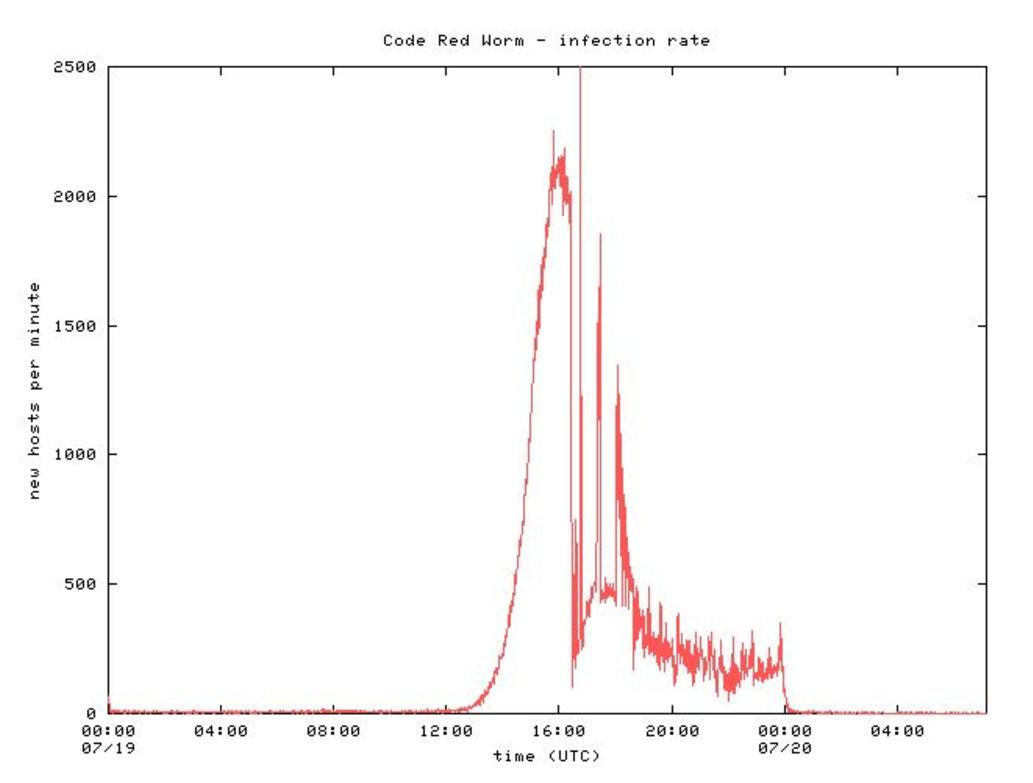
\includegraphics[width=0.95\textwidth]{images/infection_rate} % second figure itself
        \caption{tasso di infezione}
        \label{rate}
    \end{minipage}
\end{figure}
La figura ~\ref{deactivated} mostra il numero di host che hanno smesso di sondare la rete al variare del tempo e, a conferma di quanto detto sopra, tale numero era già pari a circa 200000 unità (oltre il 50\% delle infezioni totali) prima che il worm cessasse definitivamente l’attività di diffusione per procedere alla fase di attacco DDoS.\\
\begin{figure}[!hbp]
\centering
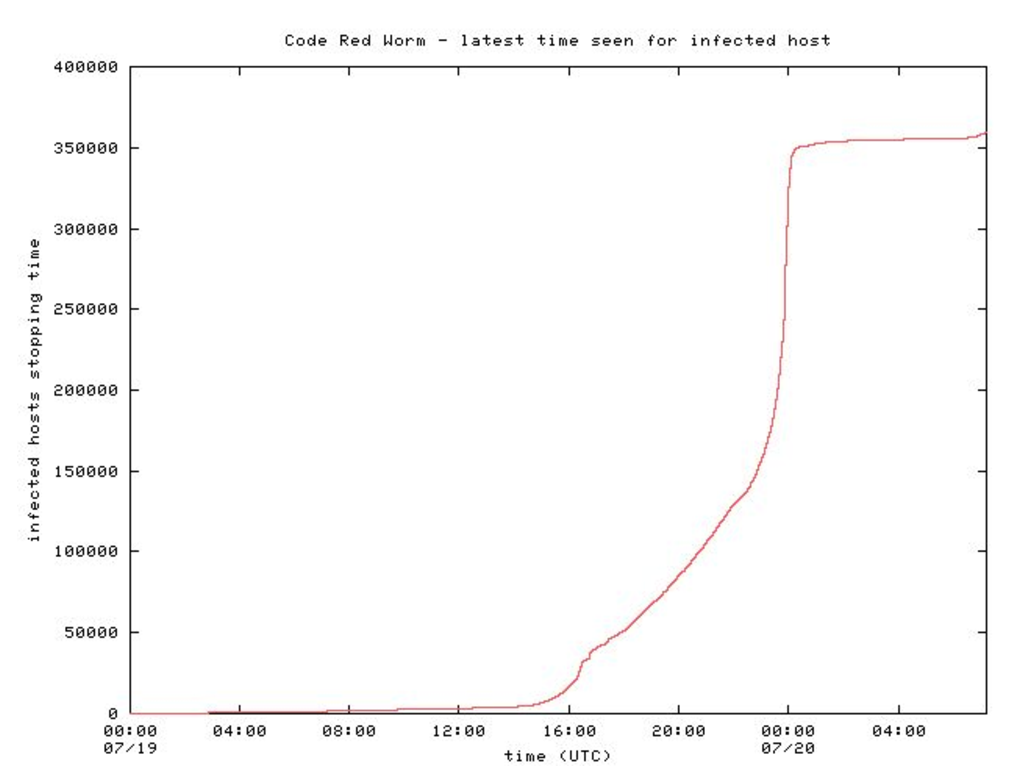
\includegraphics[width=0.7\textwidth]{images/deactivated.eps}
\caption{host "disattivati"}
\label{deactivated}
\end{figure}
Per comprendere la composizione demografica dell’utenza coinvolta, i ricercatori del CAIDA~\cite{caida} hanno esaminato i vari livelli di dominio e la locazione geografica degli host infetti.\\
La figura~\ref{domains} riassume i risultati di tale studio: per quanto riguarda i domini di primo livello la proporzione rispetta la allora attuale situazione dei web server, mentre è curioso notare che il 10\% delle macchine compromesse sono state localizzate in Korea; i principali nomi di dominio sono costituiti da server provider per infrastrutture casalinghe e piccole imprese, da qui si vede che anche queste piccole realtà hanno un ruolo rilevante riguardo la salute globale di internet.\\
\begin{figure}[!hbp]
\centering
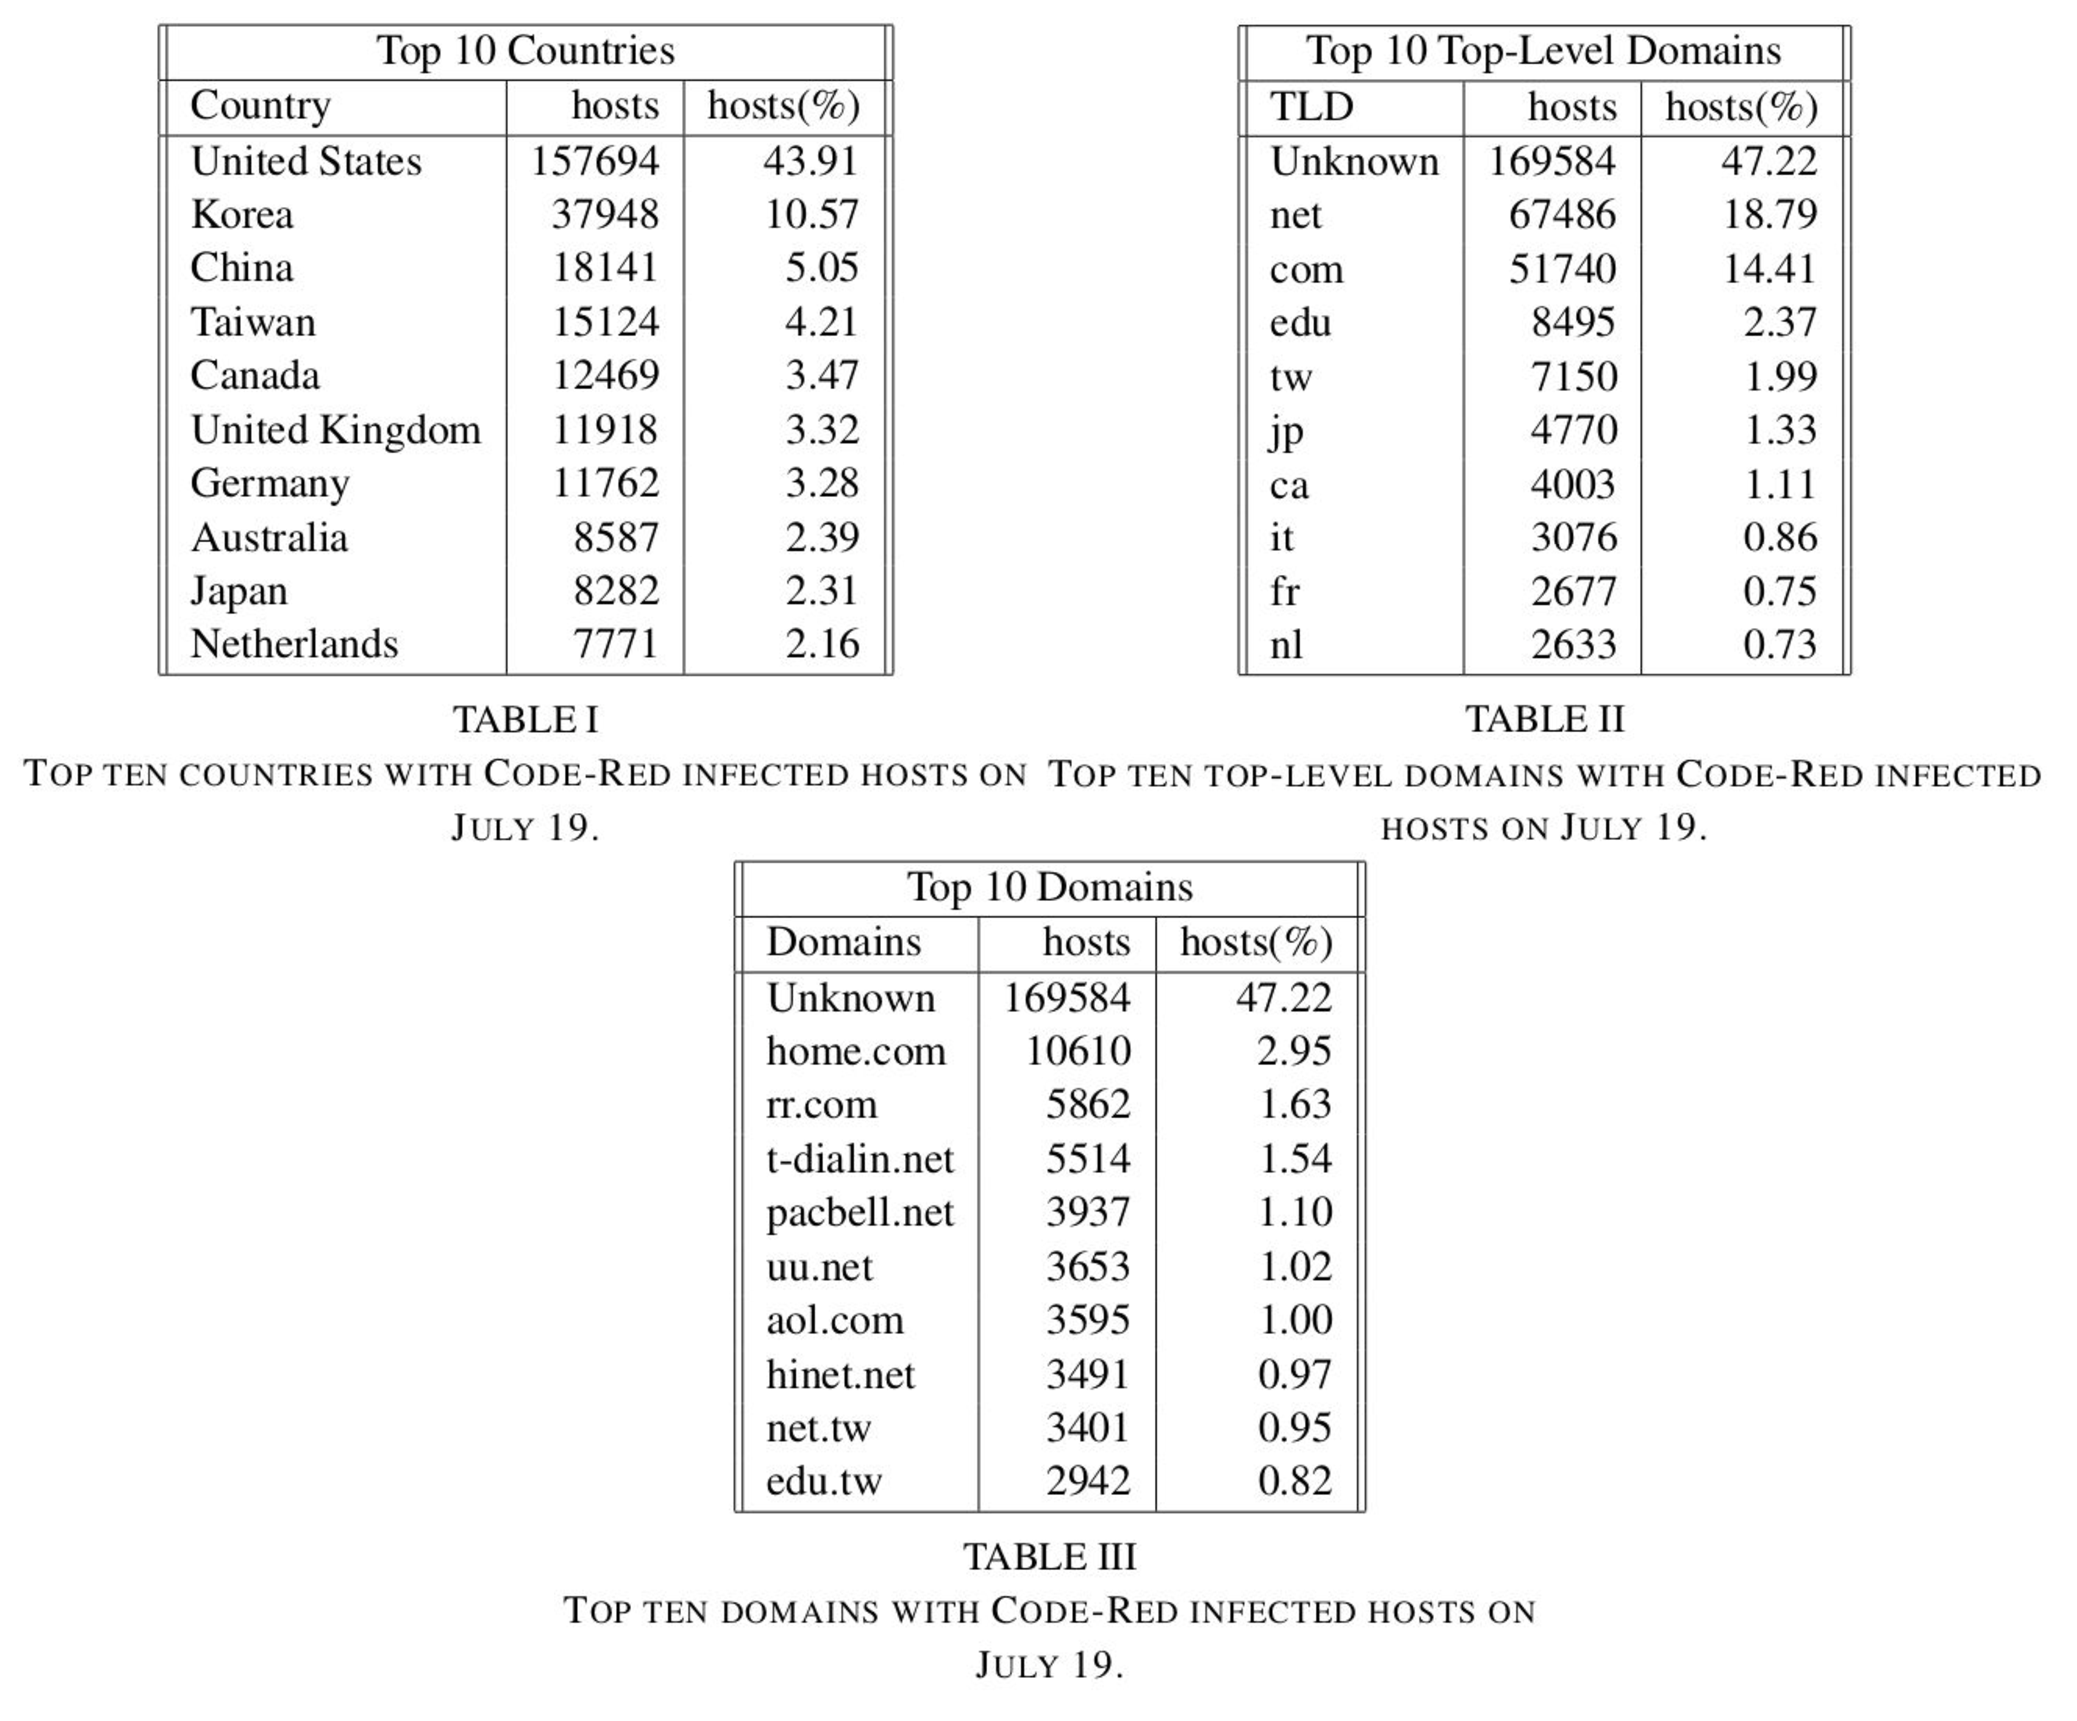
\includegraphics[width=0.8\textwidth]{images/domains.eps}
\caption{risultati analisi demografica}
\label{domains}
\end{figure}


\section{Conseguenze e impatto economico}
I principali effetti del worm Code Red furono il degradamento delle prestazioni e la perdità di stabilità dei sistemi coinvolti. Il costo globale complessivo stimato fu di 2.6 miliardi di dollari \cite{ce, sans}, di cui 1.1 miliardi impiegati nell’ispezione ed il recupero dei server ed i restanti 1.5 miliardi riguardarono le perdite di produttività a seguito dell’indisponibilità dei sistemi.\\
Quest’ultimi comprendevano non soltanto le macchine server degli utenti finali, ma anche vaste porzioni dell’infrastruttura di rete che furono completamente disabilitate, molte compagnie provider di dispositivi di rete sperimentarono un’indisponibiltà media di ben 36 ore \cite{sans}.\\
Il processo di propagazione del worm ha generato un’enorme quantità di pacchetti. Sebbene il volume di questi pacchetti era relativamente piccolo rispetto al normale traffico di rete, l’ingente quantità ha causato congestionamento e gravi problemi ad alcuni ruoter, specialmente quelli con risorse limitate. Per esempio, a causa della generazione randomica degli indirizzi IP, molti pacchetti non venivano inoltrati poiché la destinazione risultava sconosciuta, finendo così per riempire le cache ARP, esaurire la memoria e provocare il riavvio dei dispositivi \cite{cisco}.\\
La figura ~\ref{impatto} mostra il costo complessivo di Code Red in relazione agli incidenti più rilevanti del periodo \cite{ce}.

\begin{figure}[!hbp]
\centering
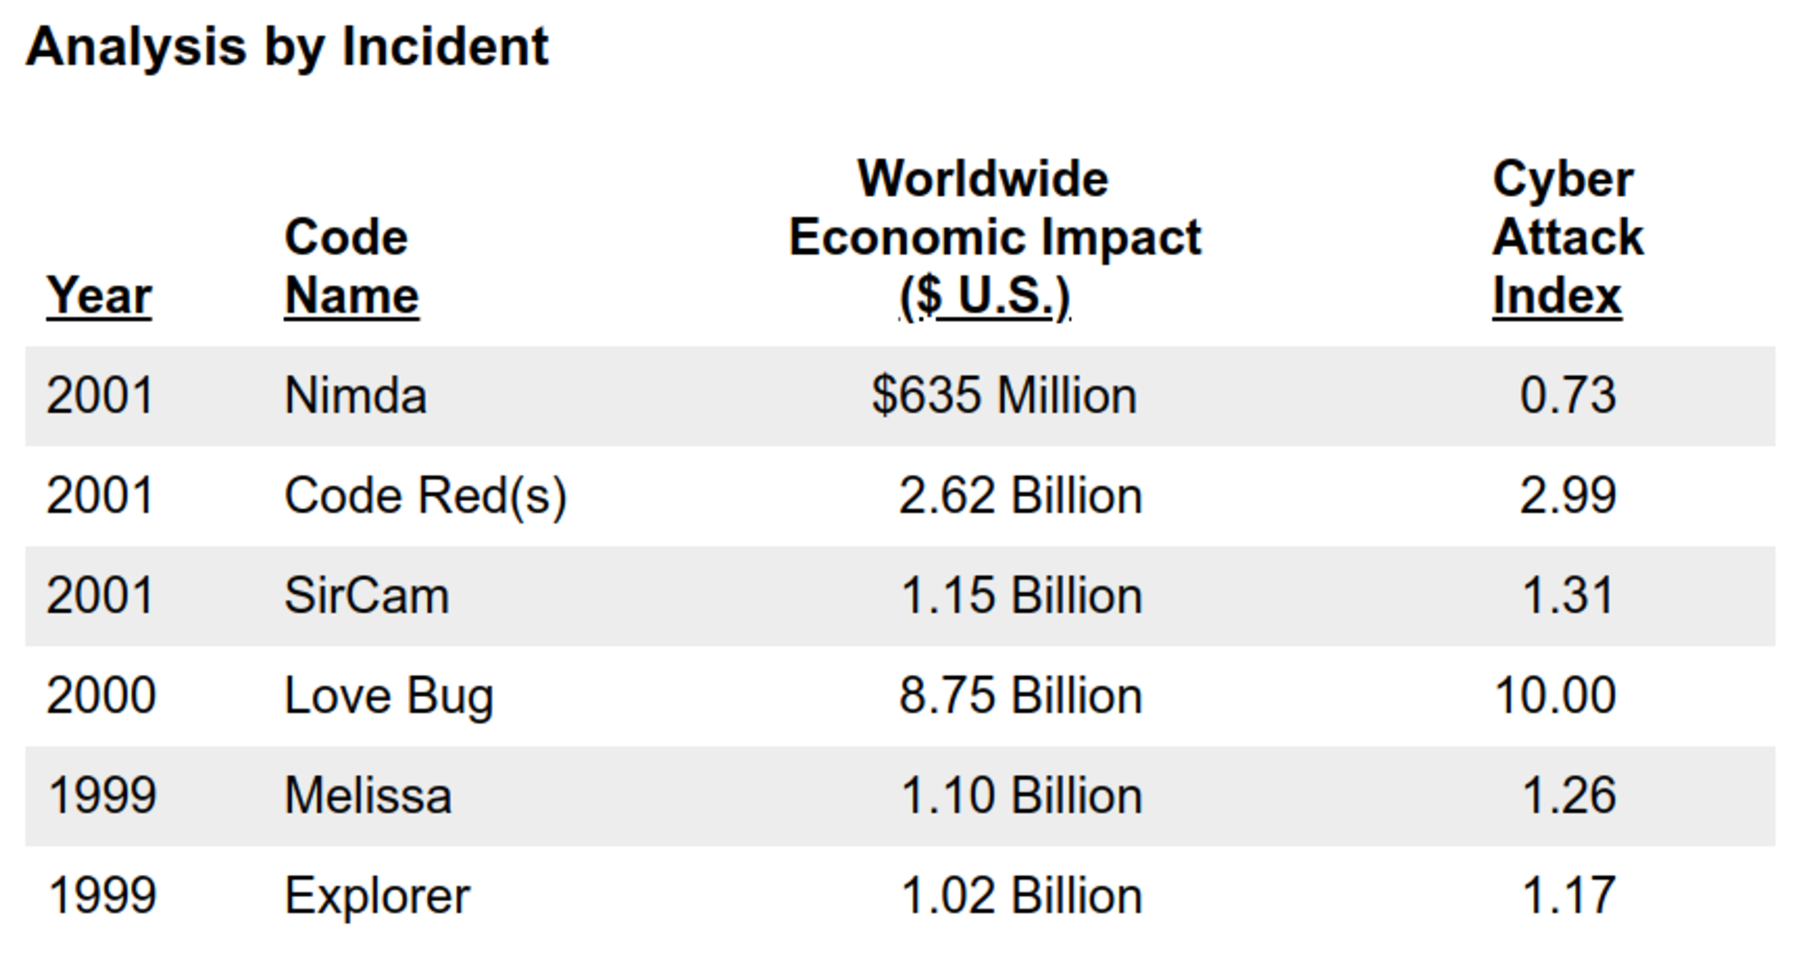
\includegraphics[width=0.5\textwidth]{images/impatto.eps}
\caption{confronto danno economico}
\label{impatto}
\end{figure}

Il sito web della Casa Bianca riuscì ad evitare conseguenze sostanzialmente “disattivando” l’indirizzo IP bersaglio dell’attacco DDoS, ovvero reindirizzando tutte le richieste non malevole verso altri indirizzi associati, questo è stato possibile perché il worm è stato progettato per inviare traffico verso un unico indirizzo IP, invece dell’intero blocco di indirizzi relativi al dominio della Casa Bianca.



\section{Esperimento: se Code Red non fosse stato scoperto}
Come appena visto Code Red ha costituito una vera e propria piaga, che si è propagata in ogni angolo del pianeta e ha causato gravi danni nonostante sia stato scoperto diversi giorni prima che la seconda versione facesse la sua comparsa ed iniziasse a diffondersi in modo efficace.\\
A fronte di ciò, abbiamo effettuato una simulazione per vedere cosa sarebbe accaduto se il worm non fosse stato scoperto, e quindi avere una misura dell’entità del danno in termini di numero di host compromessi, così poi da confrontare i risultati con il caso reale in cui la consapevolezza della presenza di tale minaccia ha spinto gli utenti ad adottare contromisure come patch, firewall, antivirus e simili.\\
Per fare questo, innanzitutto è stato necessario l’ausilio di un modello epidemico che simulasse fedelmente il comportamento ed in particolare la diffusione del worm.\\
I classici modelli per lo studio dello sviluppo epidemico, però, non sono adatti a replicare il comportamento di Code Red, perché non tengono conto delle contromisure umane intraprese durante il processo di diffusione e inoltre considerano il tasso di infezione costante nel tempo. Questi due fattori hanno portato Zou et al.~\cite{two-factor} alla derivazione del “Two Factor Worm Model” con cui hanno dimostrato tramite simulazione che i risultati approssimano bene l’andamento dei dati osservati, in particolare sono riusciti a giustificare il rallentamento delle scansioni che si è verificato appena prima il cessamento dell’attività di diffusione del worm. Tale evento, infatti, è la conseguenza della violenta propagazione su larga scala che ha provocato congestionamento e danni alla rete.\\
Le figure~\ref{tf_model} e~\ref{tf_compare} mostrano i risultati ottenuti da Zou et al., in particolare la figura~\ref{tf_compare} mostra il confronto con i dati reali osservati da Goldsmith and Eichman~\cite{gold, eich}.\\
\begin{figure}
    \centering
    \begin{minipage}{0.5\textwidth}
        \centering
        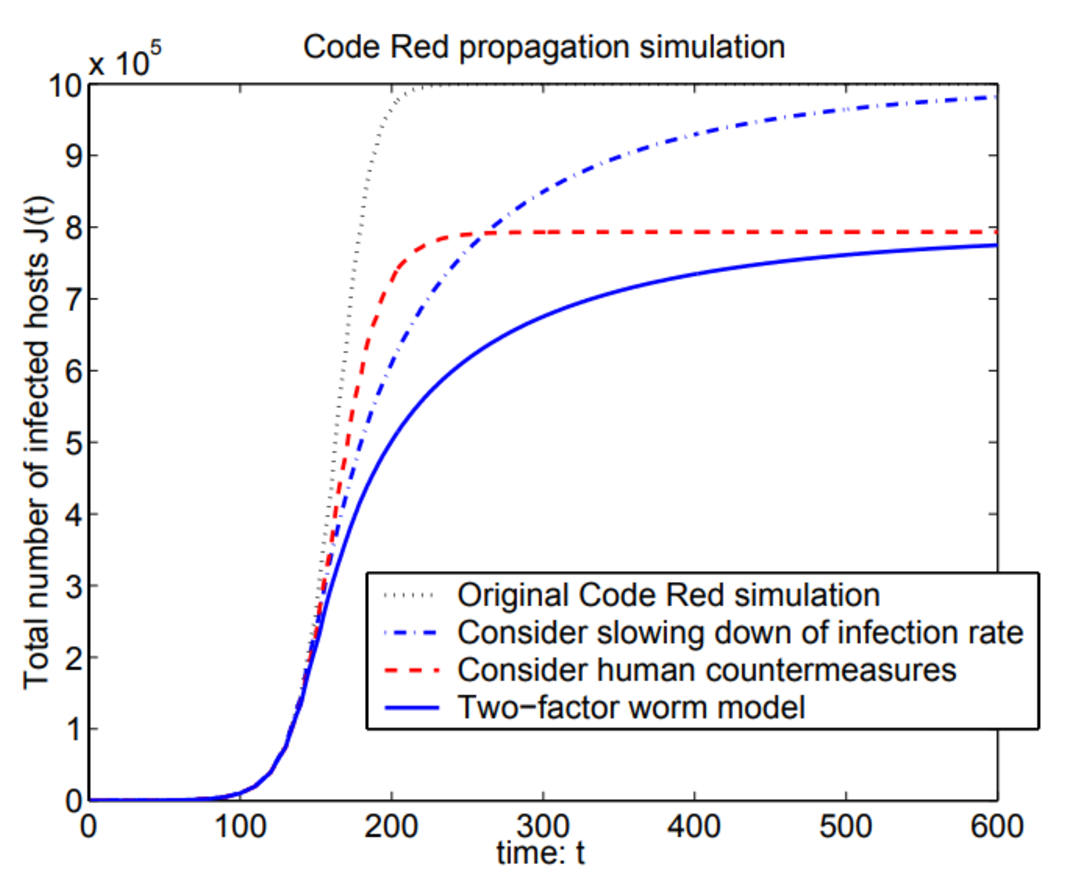
\includegraphics[width=0.95\textwidth]{images/tf_model} % first figure itself
        \caption{infezioni al variare del tempo}
        \label{tf_model}
    \end{minipage}\hfill
    \begin{minipage}{0.5\textwidth}
        \centering
        \includegraphics[width=0.95\textwidth]{images/tf_compare} % second figure itself
        \caption{confronto dati-modello}
        \label{tf_compare}
    \end{minipage}
\end{figure}
Di seguito è riportato il set di equazioni differenziali che descrivono il sistema, caratterizzanti sono il fattore $\beta(t)$ che rappresenta la frequenza di infezione variabile nel tempo, ed i fattori $R(t)$ e $Q(t)$ che costituiscono il numero di host rimossi dalla popolazione infetta a seguito di contromisure a valle del contagio, ed il numero di host rimossi dalla popolazione suscettibile (vulnerabile) a seguito di contromisure a monte, le altre variabili sono riassunte nella tabella di figura~\ref{notations}.\\
\begin{equation}
\left\{  \begin{array}{rcl} 
                dS(t)/dt &=& -\beta(t)S(t)I(t) - dQ(t)/dt, \\ 
                dR(t)/dt &=& \gamma I(t), \\ 
                dQ(t)/dt &=& \mu S(t)J(t), \\ 
                \beta(t) &=& \beta_{0}[1 - I(t)/N]^{\eta}, \\ 
                N &=& S(t) + I(t) + R(t) + Q(t), \\
                I(0) &=& I_{0} \ll N; S(0) = N -I_{0}; R(0) = Q(0) = 0; 
           \end{array}  \right.
\end{equation}
La simulazione è stata eseguita con lo stato iniziale specificato dai seguenti parametri: $N = 1000000$, $I_{0} = 1$, $\eta = 3$, $\gamma = 0.05$, $\mu = 0.06/N$ , e $\beta_{0} = 0.8/N$.\\
$I_{0}$ e $\beta_{0}$ rappresentano rispettivamente numero di host infetti e tasso di infezione iniziali, $\gamma$ e $\mu$ i tassi di rimozione, infine $\eta$ è un parametro di sensibilità che regola $\beta(t)$ in funzione di $I(t)$, sostanzialmente è un fattore che indica quanto il tasso di infezione dipende dal numero di host infetti in un certo istante di tempo, ad esempio $\eta = 0$ implica un tasso di infezione costante.\\
\begin{figure}[!hbp]
\centering
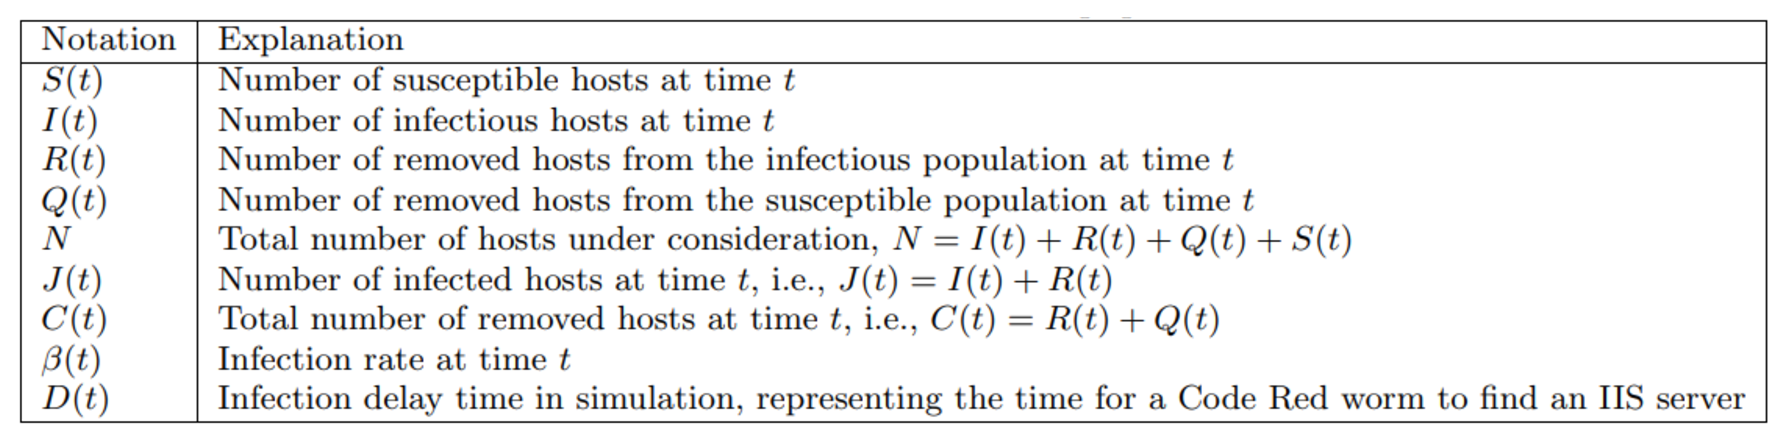
\includegraphics[width=0.95\textwidth]{images/notations.eps}
\caption{notazioni variabili del modello}
\label{notations}
\end{figure}
Il nostro studio è consistito nel semplificare il “Two Factor Model” eliminando il fattore relativo alle contromisure intraprese dagli utenti, proprio come se il worm avesse potuto agire indisturbato senza che nessuno si accorgesse della sua presenza, pertanto le variabili  R(t) e Q(t) relative agli host in stato di “rimosso” sono state annullate, ottenendo così il seguente modello semplificato:
\begin{equation}
\left\{  \begin{array}{rcl} 
                dS(t)/dt &=& -\beta(t)S(t)I(t), \\ 
                \beta(t) &=& \beta_{0}[1 - I(t)/N]^{\eta}, \\ 
                N &=& S(t) + I(t), \\
                I(0) &=& I_{0} \ll N; S(0) = N -I_{0}; 
           \end{array}  \right.
\end{equation}
La simulazione è stata realizzata tramite Simulink, a partire dalle stesse condizioni iniziali poste da Zou et al. e per un tempo di simulazione equivalente a circa 24h.\\
I risultati ottenuti (Figura~\ref{simpler}) mostrano che in 12 ore (metà tempo di simulazione) circa il 70\% degli host suscettibili sono stati infettati, approssimativamente la stessa proporzione della simulazione effettuata da Zou et al., quindi in definitiva il fatto che Code Red sia stato scoperto prima della sua violenta diffusione non ha alleviato significativamente le conseguenze in termini di macchine infettate.\\
Questo risultato mette in evidenza che di fronte ad un worm così aggressivo come Code Red, con un tasso di propagazione che ha raggiunto un picco di 2000 infezioni al minuto, le contromisure che vengono adottate a seguito dell’inizio dell’epidemia non contribuiscono a porre rimedio in maniera efficace da un punto di vista globale, ma ciò che può fare la differenza sono le contromisure preventive che vengono attuate prima degli attacchi, ovvero quelle che tendono a ridurre il numero di host potenzialmente a rischio. Quindi il vero fattore che ha favorito gli effetti devastanti del worm è stata la mancata applicazione della patch che andava ad eliminare la vulnerabilità sfruttata, nonostante fosse stata resa disponibile non poche settimane prima della comparsa della minaccia.\\
\begin{figure}[!h]
\centering
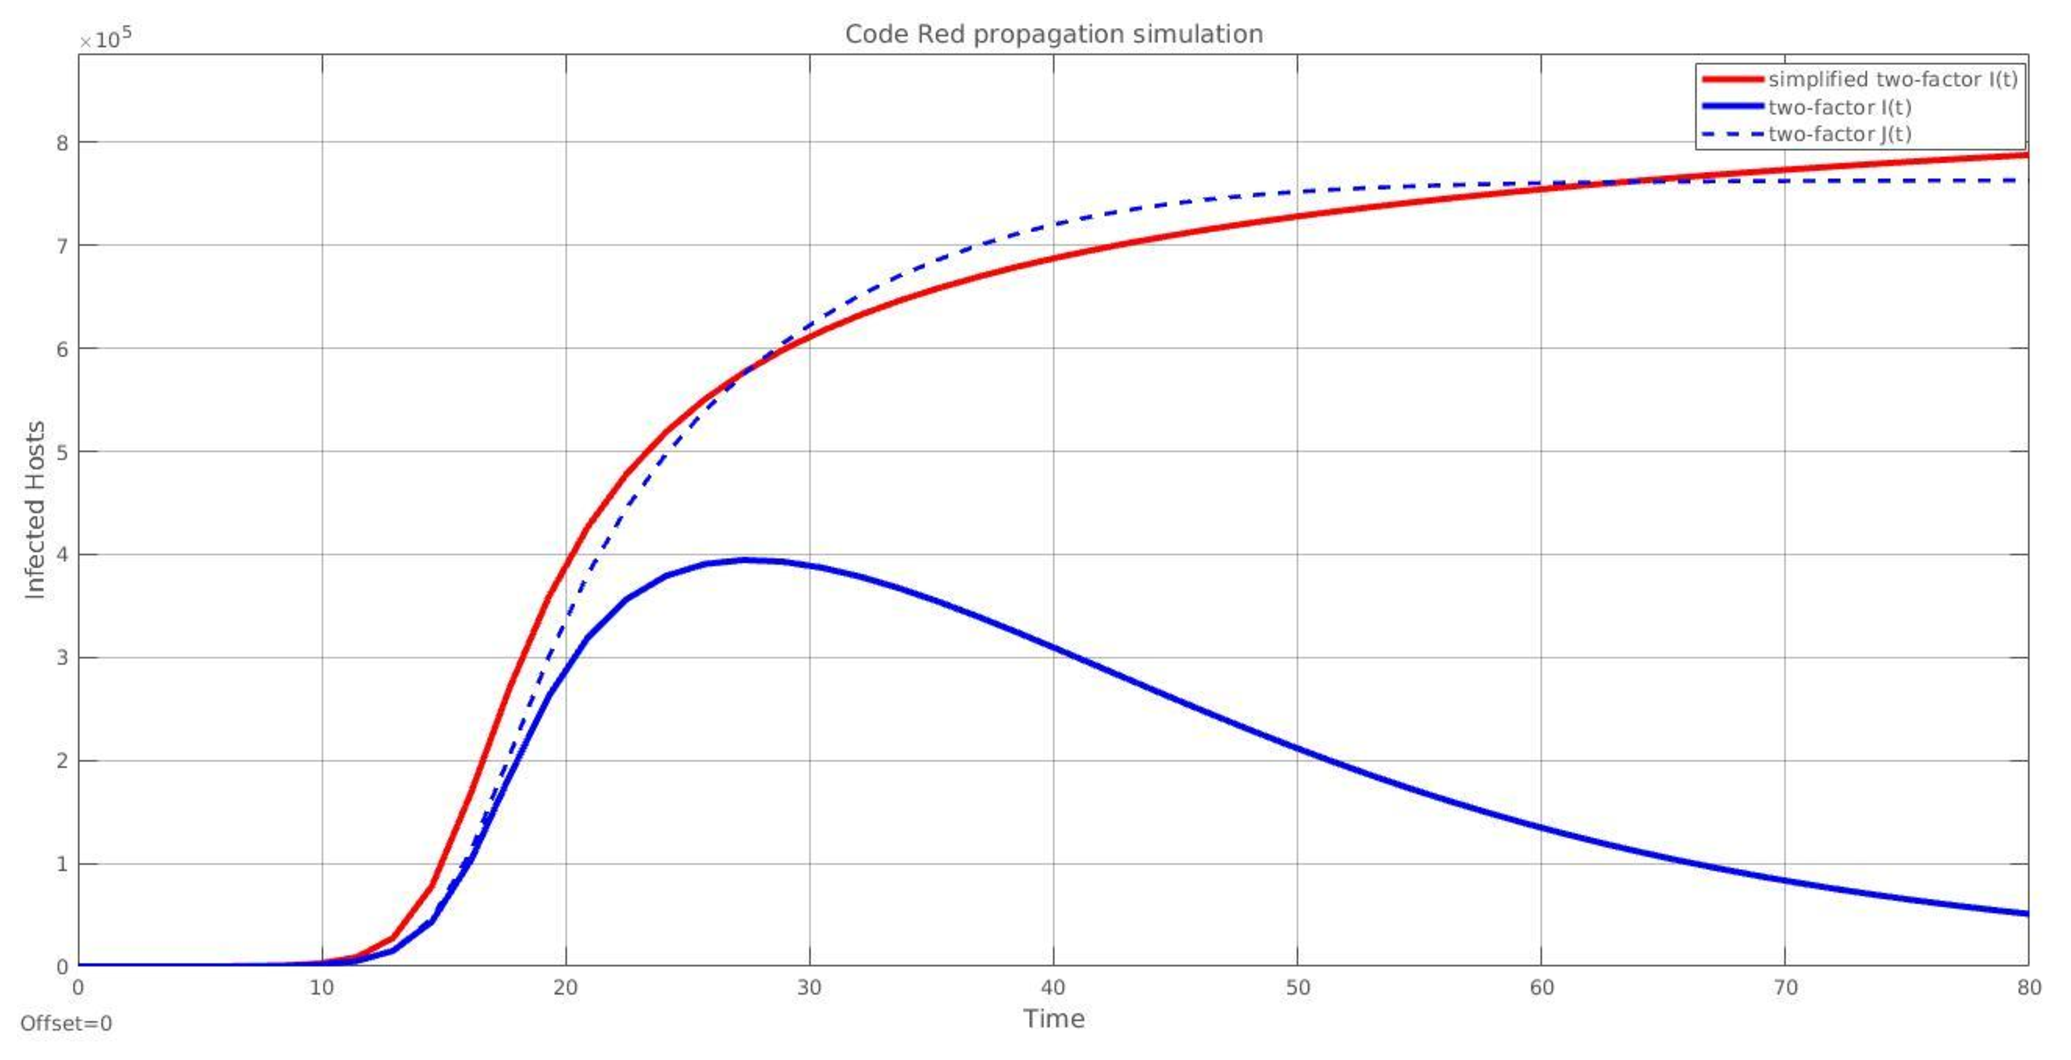
\includegraphics[width=0.95\textwidth]{images/simpler.eps}
\caption{modello semplificato vs. two-factor}
\label{simpler}
\end{figure}


\section{Contromisure}
Le contromisure possibili possono essere classificate come contromisure “a monte” e “a valle”.\\
“A monte” abbiamo:
\begin{itemize}
\item[-] la possibilità di disattivare gli script .ida e .idq nel caso in cui non fossero necessari;
\item[-] cambiare indirizzo IP per evitare l’attacco DDoS. Nello specifico è stata la soluzione adottata dalla Casa Bianca al momento dell’attacco;
\item[-] il download della patch che va ad inserire il controllo sull’input mancante, in modo da eliminare completamente la vulnerabilità presente.
\end{itemize}
“A valle” ci sono invece dei prodotti software utili per scansionare il dispositivo ed eventualmente eliminare il worm trovato. Questi sono “FixCodeRed” rilasciato dalla Symantec e “CodeRedScanner” rilasciato proprio dalla Eye Digital Security.\\
Queste contromisure sono state effettivamente adottate nel periodo dell’attacco e hanno contribuito, almeno in parte, alla riduzione della diffusione e delle conseguenze dell’attacco. Non sono però le uniche contromisure valide, anzi ce ne sono altre che avrebbero avuto un ottimo impatto nella difesa da Code Red, alcune delle quali ne avrebbero addirittura impedito una diffusione così elevata.\\
Le contromisure che abbiamo individuato sono state:
\begin{enumerate}
\item Contenimento automatizzato dei worm
\item SSL - Security Socket Layer
\item ACL - Access Control List
\item Reverse Proxy
\item IDS - Intrusion Detection System
\item WAF - Web Application Firewall
\end{enumerate}
%%%%%%%%%%%%%%%%%%%%%%%%%%%%%%%%%%%%%%%%%%%%%%%%%%%%%%%%%%%%%%%%%%%%%%%%%%%%%
\subsection{Contenimento automatizzato dei worm}
Il contenimento automatizzato è una tecnica ideata dai ricercatori Sellke, Shroff e Bagchi~\cite{selke} che consiste nel blocco o nel rallentamento della comunicazione tra host infetti e host non infetti, impedendo ad un generico worm a scansione randomica di diffondersi sin dalle prime fasi del contagio.\\
L’idea principale è quella di limitare il numero totale di distinti indirizzi IP contattati da un singolo host nell’arco di un lungo periodo di tempo (settimane o anche giorni), detto ciclo di contenimento, in modo tale da ottenere una probabilità di estinzione $\pi$ prossima a 1.\\
La seguente proposizione fornisce la condizione necessaria e sufficiente affinché l’estinzione si verifichi con certezza:\\
%%%%%%%%
\newtheorem{prop}{Proposizione}
\begin{prop}
Sia p la densità di probabilità degli host suscettibili e M il numero massimo di scansioni per host, allora:
\begin{displaymath}
    \pi = 1  \Leftrightarrow  M \le 1/p 
\end{displaymath}
\end{prop}
%%%%%%%%%
L’implicazione pratica di questa proposizione è che limitando il numero totale di scansioni per host a non più di $1/p$, la diffusione del worm sarà eventualmente contenuta entro un certo numero di generazioni.\\
La densità $p$ è la probabilità di trovare un host vulnerabile ad ogni scansione ed è pari a $V/232$ dove $V$ corrisponde al numero di host vulnerabili e $2^{32}$ è la dimensione dello spazio degli indirizzi IPv4.\\
Se si assume per semplicità che il numero di host vulnerabili a Code Red era almeno di $360000$ unità, si ottiene un valore di $p$ pari a $8.5 x 10^{-5}$, e di conseguenza il numero massimo di scansioni $M$ è pari a $11930$.
La figura~\ref{auto} mostra i risultati dello studio di Selke et al. in cui si evidenzia come con un valore di $M = 10000$, il numero totale di host infetti risulti essere inferiore a $360$ unità con una probabilità del 99\%, tale numero corrisponde a circa lo 0.1\% del totale degli host vulnerabili all’epoca.\\
\begin{figure}[!h]
\centering
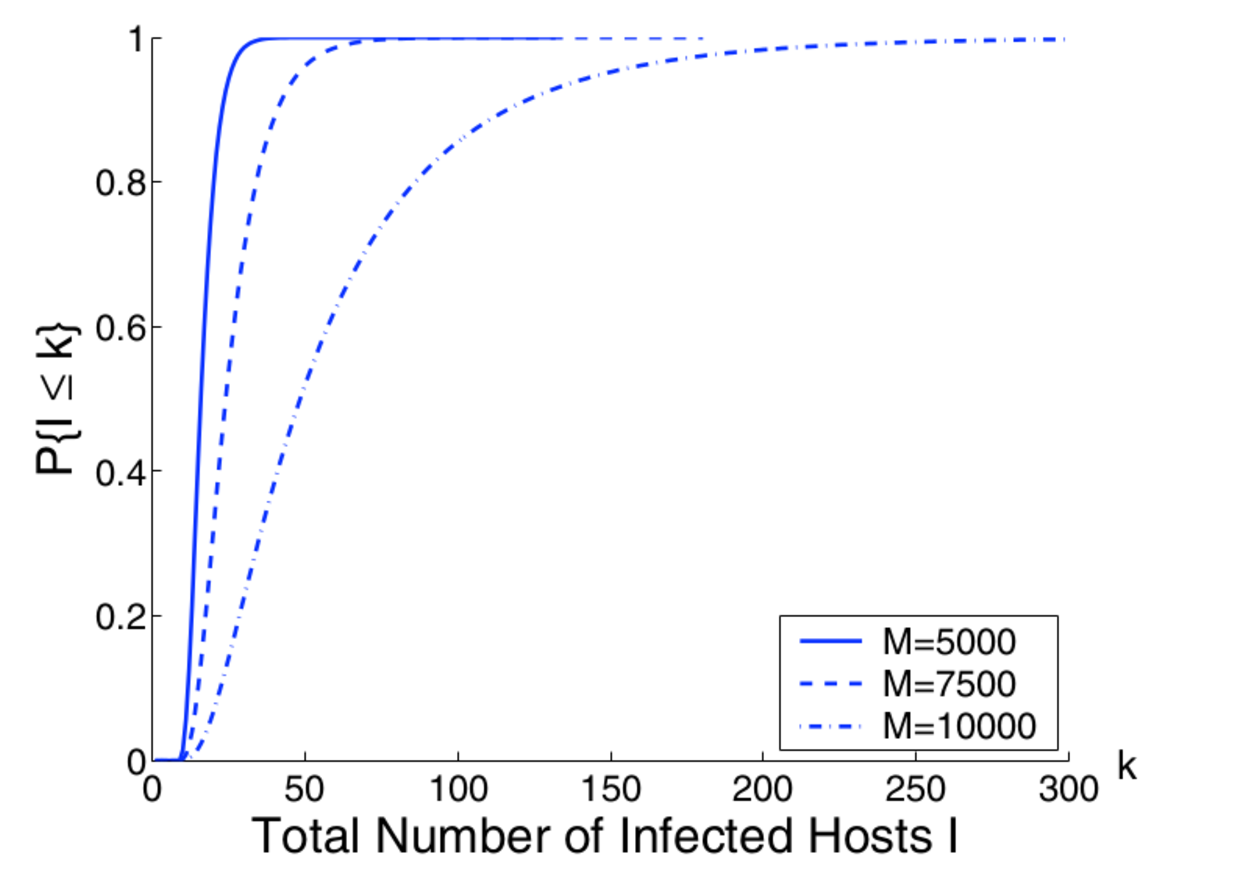
\includegraphics[width=0.6\textwidth]{images/auto.eps}
\caption{distribuzione cumulativa infezioni}
\label{auto}
\end{figure}
In sintesi la strategia si compone dei seguenti passi:
\begin{enumerate}
\item Imporre un limite M al numero di distinti indirizzi IP che un host può contattare in un ciclo di contenimento. All’inizio di ogni ciclo inizializzare il contatore
\item Incrementare il contatore ogni qualvolta viene contattato un nuovo indirizzo IP
\item Se un host raggiunge il valore di soglia prima del termine del ciclo di contenimento viene isolato, analizzato ed eventualmente reso immune prima che venga reintrodotto in rete, dopodiché il contatore viene riazzerato.
\item al termine del ciclo il contatore viene resettato
\end{enumerate}
I vantaggi del contenimento automatizzato sono i seguenti:
\begin{itemize}
\item[-] È una soluzione applicabile a livello di singolo host, quindi semplifica la fase di deploy, inoltre a seconda delle necessità può essere applicata a router di rete impostando un valore di soglia globale per tutti i gli host connessi.
\item[-] Il sistema di contenimento è adatto a worm aventi qualsiasi velocità di scansione, senza conoscerne la signature.
\item[-] Non interferisce con il normale traffico scambiato, poiché dallo studio di Selke et al. emerge che il 97\% degli host contatta meno di 100 indirizzi IP differenti durante un ciclo di contenimento di 30 giorni, soltanto una piccola percentuale raggiunge i 4000 host, pertanto è sufficiente imporre un lower bound al numero di scansioni ponendo M > 5000. Il valore di soglia può comunque essere reso adattivo in base alla normale frequenza di scansionamento dell’host in questione.
\end{itemize}
%%%%%%%%%%%%%%%%%%%%%%%%%%%%%%%%%%%%%%%%%%%%%%%%%%%%%%%%%%%%%%%%%%%%%%%%%%%%%
\subsection{SSL - Security Socket Layer}
L’SSL è un protocollo degli anni ‘90, che ha preceduto il TLS (Transport Layer Security) . Per fornire un meccanismo di autenticazione e cifratura usa una combinazione di cifratura simmetrica e a chiave pubblica. Include i protocolli:
\begin{itemize}
\item[Handshake], in cui viene stabilita una connessione SSL e negoziati algoritmi e sistemi crittografici usati;
\item[Record], in cui si definisce come avviene lo scambio dei dati, quali sono i dati da scambiare e come autenticarli e decifrarli.
\end{itemize}
Siamo interessati al protocollo di Handshake perché implicato direttamente nella fase di diffusione del worm. Secondo tale protocollo:
\begin{itemize}
\item[-] il server presenta il suo certificato digitale al client (certificato X.509);
\item[-] l’autenticazione usa la cifratura a chiave pubblica per validare il certificato digitale;
\item[-] finita l’autenticazione, le parti stabiliscono la cifratura e una chiave di sessione (viene fornita confidenzialità e integrità dei dati).
\end{itemize}
Quindi per abilitare l’SSL, l’admin del web server deve deve ottenere un certificato digitale da una terza parte, cioè un “Autorità di Certificazione”.\\
SSL sarebbe stato la soluzione migliore per evitare la diffusione di Code Red, in quanto questo durante la fase di diffusione andava ad evitare tutti i dispositivi con SSL attivo. L’obiettivo del worm era di raggiungere la più alta diffusione possibile, per poter ottenere un attacco più consistente possibile verso la Casa Bianca.\\
Code Red per infettare nuovi dispositivi agiva nel seguente modo: stabiliva una connessione con un nuovo dispositivo, procedeva con essa e si fermava solo all’inizio di una eventuale fase di handshake, in quanto era sintomo del protocollo SSL attivo, dunque interrompeva la connessione e andava alla ricerca di un nuovo dispositivo da infettare.\\
SSL è un modo semplice per proteggersi da attacchi DDoS, perchè è semplice da implementare e relativamente economico. Richiede solo di possedere un certificato digitale (la cui spesa è di \$349/anno da Verisign Corp.) e una configurazione appropriata.\\
Da un sondaggio del 2001 è emerso purtroppo che meno di 122.000 web server avevano SSL valido, contro i 27 milioni di server attivi (meno della metà dell’1\%). Per questo motivo Code Red non ha trovato freni durante la sua diffusione, e questo è il motivo dell’ingente quantità di macchine che è riuscito ad infettare nel giro di poche ore. Una maggiore attenzione da parte degli amministratori dei server web avrebbe impedito una diffusione cosi estesa, evitando i conseguenti danni registrati.\\
%%%%%%%%%%%%%%%%%%%%%%%%%%%%%%%%%%%%%%%%%%%%%%%%%%%%%%%%%%%%%%%%%%%%%%%%%%%%%
\subsection{ACL - Access Control List}
L’ACL serve per monitorare il traffico, filtrarlo e bloccare un eventuale worm/attacco DDoS. Ne esistono sia per il livello WAN che LAN e sono customizzabili dall’admin. Il loro controllo si basa sull’indirizzo IP del mittente, quindi ogni interfaccia di rete va dotata di un ACL sia per il traffico in ingresso che per quello in uscita.\\
L’ACL rappresenta una misura preventiva per l’attacco e non ha impatto sulle performance del router. L’idea è quella di creare un perimetro entro cui il traffico malevolo non possa entrare, impedendo ai sistemi infetti di attaccare altri sistemi vulnerabili o altre sottoreti. Per tale motivo andrebbero applicate all’interfaccia più vicina alla sorgente di traffico, in modo da avere una maggiore efficienza.\\
Le ACL devono proteggere un server filtrando il traffico, ma devono permette comunque che esso sia accessibile dall’esterno. Quindi le ACL poste al confine delle DMZ devono permettere alle richieste di arrivare ai server, impedendo però che questi siano direttamente accessibili.\\
La strategia per contrastare la diffusione di un worm, o un attacco di tipo DDoS, è quello di isolarlo il prima possibile e procedere alla sua rimozione. Proteggendo la rete con le ACL la minaccia resta confinata in una porzione della rete, e li può essere combattuta ed eliminata con un effort minore rispetto a dopo la sua diffusione.\\
L’impatto di un eventuale attacco DDoS è limitato dal perimetro di rete e gli attaccanti non riescono a raggiungere, ed utilizzare, i dispositivi interni al perimetro a favore dell’attacco. Si evitano sia l’overload dei sistemi che l’interruzione dei servizi basati su tali dispositivi, e di conseguenza che le risorse di rete vengano consumate da traffico non desiderato.\\
Lo svantaggio nell’utilizzo delle ACL è il fatto di doverne usare più di una per aumentare il grado di protezione. Inoltre vanno aggiornate con le vulnerabilità correnti prima dell’eventuale inizio di un attacco, altrimenti non sarebbero in grado di isolarlo tempestivamente.\\
\begin{figure}[!h]
\centering

\includegraphics[width=0.6\textwidth]{images/acl.eps}
\caption{esempio di acl}
\label{acl}
\end{figure}
%%%%%%%%%%%%%%%%%%%%%%%%%%%%%%%%%%%%%%%%%%%%%%%%%%%%%%%%%%%%%%%%%%%%%%%%%%%%%
\subsection{Reverse Proxy}
Un server “proxy” è un server che fa da intermediario tra un client ed un altro server, usato per disaccoppiare l’accesso al web da un browser. Le richieste del client non sono gestite direttamente dal server di destinazione ma vengono gestite da un server intermedio.\\
Un server “reverse proxy” viene usato invece come intermediario tra la rete pubblica ed i server ad esso associati. La fase di “three hand handshake” viene eseguita con il reverse proxy ed è lui che inoltrerà la richiesta al web server richiesto.\\
Il reverse proxy è una soluzione adatta per mitigare l’effetto di un attacco DdoS, perchè il traffico malevolo (destinato ad un singolo server) viene distribuito su più reverse proxy.\\
Lo svantaggio nel suo utilizzo è legato al suo costo di mantenimento, nello specifico delle tabelle di configurazione relative ai server web gestiti dal reverse proxy.\\
\begin{figure}[!h]
\centering
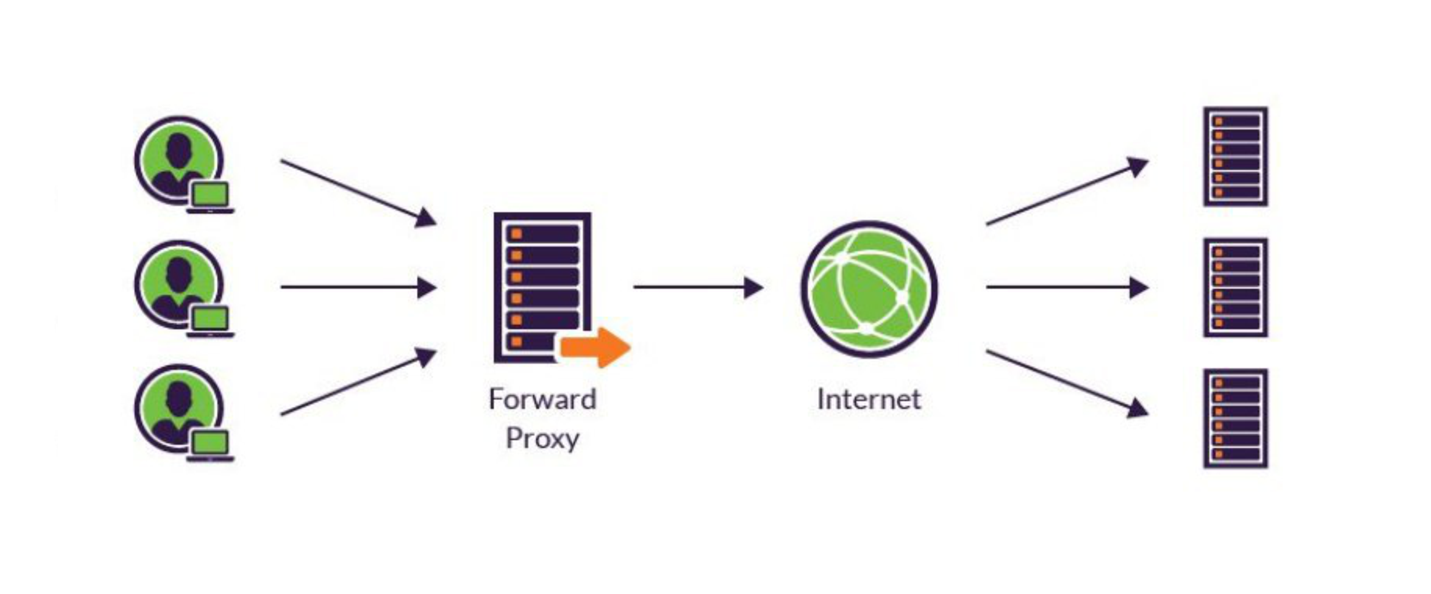
\includegraphics[width=0.6\textwidth]{images/proxy_1.eps}
\caption{esempio forward proxy}
\label{fproxy}
\end{figure}
\begin{figure}[!h]
\centering
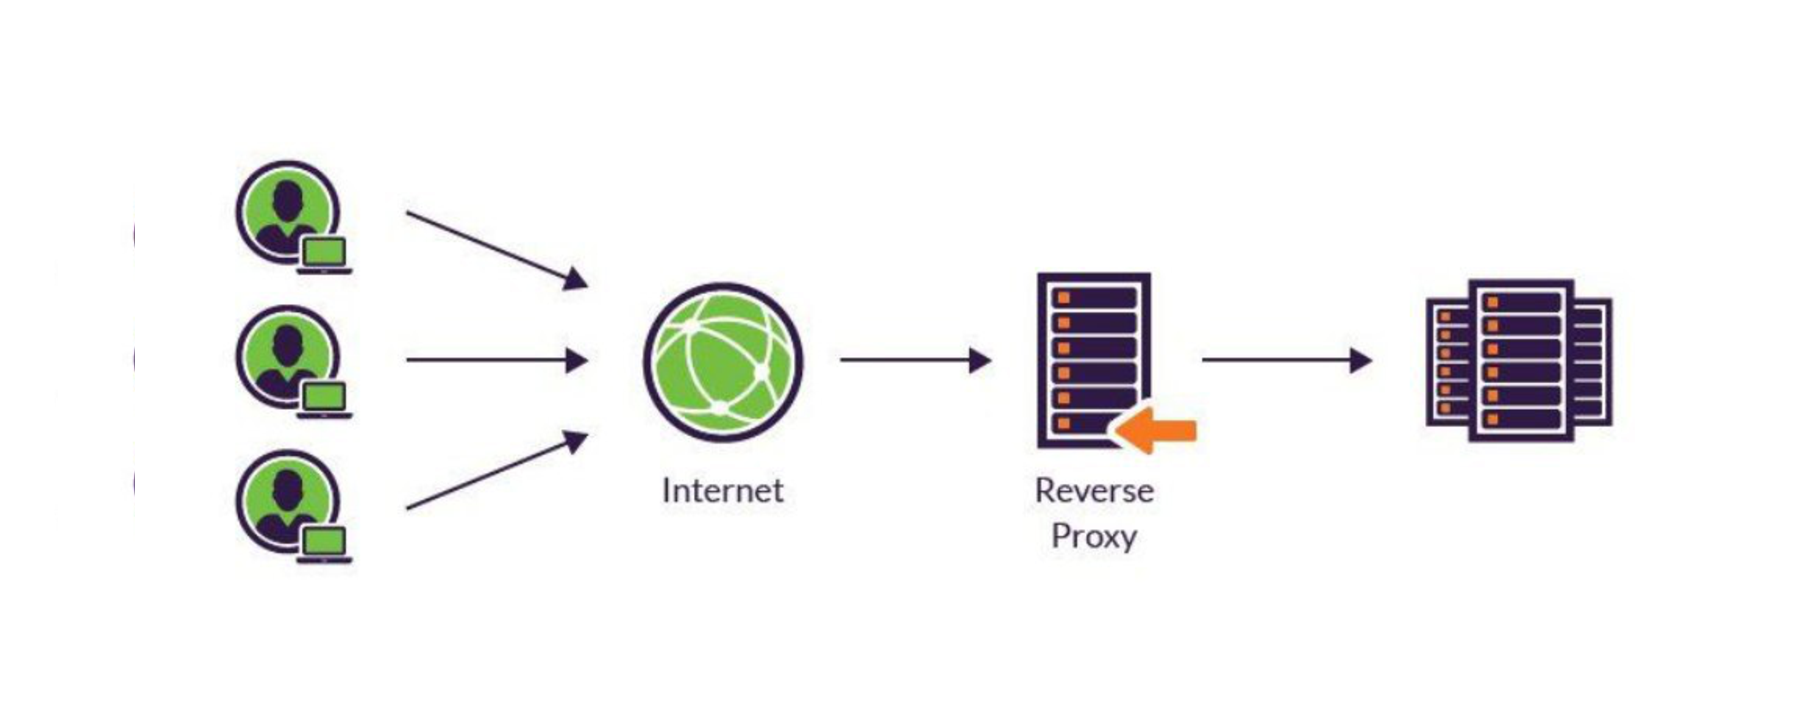
\includegraphics[width=0.6\textwidth]{images/proxy_2.eps}
\caption{esempio reverse proxy}
\label{rproxy}
\end{figure}
%%%%%%%%%%%%%%%%%%%%%%%%%%%%%%%%%%%%%%%%%%%%%%%%%%%%%%%%%%%%%%%%%%%%%%%%%%%%%
\subsection{IDS - Intrusion Detection System}
L’ IDS è un dispositivo hardware o software che colleziona informazioni sul server e/o la rete per analizzarle e determinare la presenza di un attacco o un intrusione.\\
Tale sistema può essere “network-based” se monitora il traffico sul suo segmento di rete, o “host-based” se monitora il software su un server.\\
Può agire a livello di rete, di trasporto o di applicazione ed è in grado di segnalare eventuali anomalie all’admin, o eseguire operazioni in modo autonomo.\\
Per svolgere il suo compito usa come meccanismi:
\begin{itemize}
\item[-]verifica dei log
\item[-]controllo dell’integrità dei file locali
\item[-]monitoring dei pacchetti in arrivo
\end{itemize}
Tale sistema può essere usato in modo molto efficace per contrastare il worm Code Red durante la sua fase di attacco, cioè bloccando l'attacco DdoS sulla porta 80 di un web server. A tal proposito il sistema analizza in real-time le richieste in arrivo al web server, attraverso due tecniche dette “anomaly detection” e “misuse detection”:\\
anomaly detection, confronta le “signature action” con i pattern di intrusione noti che sono contenuti in un database;
misure detection, osserva le operazioni eseguite dal server e costruisce un suo profilo di “utilizzazione normale”, in modo da poter riconoscere operazioni e utilizzi del server diversi da quelli soliti.\\
L’IDS risulta essere molto efficace nel prevenire un attacco, con un elevata affidabilità e ottime performance. Ciò è possibile perché, sfruttando i pattern di attacchi noti, riesce a identificare tempestivamente l’attacco su una macchina, durante le fasi iniziali dell’attacco stesso, riuscendo quindi a impedirne la realizzazione.\\
Lo svantaggio è legato a due fattori principali: il primo è la complessità del sistema stesso, che rende necessaria la presenza di un team di professionisti per configurarlo e utilizzarlo; il secondo è rappresentato dall’utilizzo dei pattern nel database. Infatti quest’ultimo va tenuto sempre aggiornato inserendo manualmente i pattern degli attacchi più recenti, in modo da poterli sfruttare a proprio favore. Inoltre, usando i pattern di attacchi noti, il sistema non è in grado di rilevare un attacco “nuovo” basato su un pattern che non è presente nel database.\\
%%%%%%%%%%%%%%%%%%%%%%%%%%%%%%%%%%%%%%%%%%%%%%%%%%%%%%%%%%%%%%%%%%%%%%%%%%%%%
\subsection{WAF - Web Application Firewall}
Il WAF è un firewall che, a differenza dei firewall di rete, agisce a livello applicativo evitando l’utilizzo delle vulnerabilità di un applicazione. Esso agisce filtrando, monitorando ed eventualmente bloccando il traffico HTTP malevolo.\\
Inoltre ha il vantaggio di essere “customizzabile”, permettendoci di creare un livello di protezione “ad-hoc” per ogni nostra applicazione.\\
Il WAF è una valida alternativa per bloccare/mitigare l’attacco DdoS di Code Red, impedendo che questo possa “bloccare” il target dell’attacco. Infatti degli esperimenti~\cite{sans-acl} del 2004 hanno dimostrato che con soli 500 pacchetti/secondo si poteva bloccare un web server, mentre ne servivano addirittura 14.000 al secondo per riuscire a bloccare un firewall.\\
Utilizzare il WAF ci permette di massimizzare il rilevamento di attacchi noti e non, grazie alla sua analisi dei pacchetti a livello applicativo. Inoltre ha il vantaggio di un impatto minimo sulle performance di rete.\\
Per poter assicurare una maggiore efficacia va usato in combinazione ad un firewall di rete o un IDS. Questo perché il WAF si occupa esclusivamente di una protezione a livello applicativo, lasciando di fatto scoperta una protezione di livello di rete. L’uso di un apposito firewall di rete è una soluzione economica e di facile realizzazione, mentre nel caso ci sia bisogno di una protezione più elevata è utile l’installazione di un più complesso, e costoso, dispositivo IDS.\\


\section{Conclusioni}
La prima osservazione da fare riguardo il worm Code Red è la velocità con cui è riuscito a diffondersi, almeno nella sua seconda versione. I confini fisici e geografici hanno perso di significato davanti ad un attacco di questa portata, e in meno di 14 ore più di 359,104 macchine erano state compromesse.\\
Un secondo aspetto da evidenziare è che le macchine gestite da utenti comuni in ambito domestico, o da piccole imprese, sono parte integrante della solidità di Internet globale. Queste sono spesso gli host più vulnerabili e possono essere attaccati con facilità da un attaccante, diventando una porta di accesso verso tutti gli altri host e quindi mettendo a rischio l’intera rete.\\
Il caso studiato del worm Code Red è un ottimo esempio di questa situazione, e mette in risalto un ulteriore aspetto che è purtroppo molto diffuso ed è alla base di altri attacchi informatici: la negligenza degli utenti. Gli utenti medi della rete tendono a dare poca importanza a molti aspetti della sicurezza informatica, anche di semplice tipo, come potrebbe essere la buona gestione delle proprie password, esponendo se stessi e quindi tutto il resto della rete a possibili attacchi. Nel caso di Code Red abbiamo visto, tra le contromisure attuabili, il protocollo SSL, che è un esempio perfetto di quanto appena detto. Esso avrebbe evitato la diffusione di Code Red, e quindi tutte le conseguenze economiche dell’attacco (che ricordiamo essere state stimate intorno ai 2.6 miliardi di dollari) se fosse stato adottato da un’elevata quantità di utenti. Eppure nonostante il suo costo praticamente irrisorio, al momento dell'attacco meno della metà dell’1% degli utenti disponeva di tale protocollo attivo, e questo è uno dei motivi per cui Code Red non ha trovato freni nella sua diffusione planetaria.\\
Come visto le possibili contromisure non sono poche e risultano essere efficaci per arginare o bloccare Code Red sul nascere della sua diffusione. Le ACL attualmente sarebbero una soluzione ottima dato che il pattern di Code Red è ormai noto, ma nel 2001 non sarebbero state troppo di aiuto. La soluzione più efficace per evitare la diffusione e bloccarla sul nascere sarebbe di sicuro la più costosa, cioè l’utilizzo di un sistema IDS, anche se visto il suo costo di configurazione e di gestione lo renderebbe applicabile a zone limitate della rete.\\
Vista l’impossibilità di riconoscere un pattern sconosciuto e i costi molto elevati, la soluzione migliore per poter mitigare la diffusione del worm e un attacco DDoS, sia da un punto di vista realizzativo che economico, potrebbe essere rappresentata dall’uso di firewall, sia a livello di rete che applicativo, per poter filtrare il traffico ed evitare il carico diretto dell’attacco sul dispositivo target.\\
Per evitare la diffusione del worm invece, il protocollo SSL resta una delle soluzioni più efficaci ed economiche. 
Infine non andrebbe dimenticato il contenimento automatizzato, che nonostante sia applicabile soltanto a worm che eseguono scansioni randomiche, rimane comunque una soluzione flessibile, poco invasiva e soprattutto che non ha bisogno di conoscere le signature di eventuali minacce come Code Red.\\


\newpage
\begin{thebibliography}{99}

\bibitem{eeye} 
\emph{``ANALYSIS: .ida "Code Red" Worm''}
eEye. July 17, 2001\\
\url{https://web.archive.org/web/20110722192419/http://www.eeye.com/Resources/Security-Center/Research/Security-Advisories/AL20010717}

\bibitem{bullet}
\emph{``Microsoft Security Bulletin MS01-033 - Critical''}
Microsoft. June 18, 2001\\
\url{https://docs.microsoft.com/en-us/security-updates/securitybulletins/2001/ms01-033}

\bibitem{caida} Moore, David \& Shannon, Colleen \& Brown, Jeffery. 
\emph{``Code-Red: a case study on the spread and victims of an Internet worm''}
CAIDA.\\
\url{http://www.caida.org/publications/papers/2002/codered/codered.pdf}

\bibitem{two-factor} Cliff Changchun Zou, Weibo Gong, Don Towsley.
\emph{``Code Red Worm Propagation Modeling and Analysis.''}
Dept. Electrical \& Computer Engineering Univ. Massachusetts Amherst, MA\\
\url{http://www.cs.ucf.edu/~czou/research/codered.pdf}

\bibitem{selke} Sarah Sellke, Ness B. Shroff, and Saurabh Bagchi.
\emph{``Modeling and Automated Containment of Worms.''}
School of Electrical and Computer Engineering Purdue University\\
\url{https://ieeexplore.ieee.org/document/4358715/}

\bibitem{ce}
\emph{``Malicious Code Attacks Had \$13.2 Billion Economic Impact in 2001.''}
Computer Economics. September, 2002\\
\url{https://www.computereconomics.com/article.cfm?id=133}

\bibitem{sans} Schauer, Renee C..
\emph{``The Mechanisms and Effects of the Code Red Worm.''}
Sans Institute. 2001\\
\url{https://www.sans.org/reading-room/whitepapers/dlp/the-mechanisms-and-effects-of-the-code-red-worm-87}

\bibitem{cisco}
\emph{``Code Red Worm - Customer Impact.''}
Cisco. July 20, 2001\\
\url{https://tools.cisco.com/security/center/content/CiscoSecurityAdvisory/cisco-sa-20010720-code-red-worm}

\bibitem{eich} K. Eichman.
\emph{``Possible CodeRed Connection Attempts.''}
July 20, 2001\\
\url{http://lists.jammed.com/incidents/2001/07/0159.html}

\bibitem{gold} D. Goldsmith. 
\emph{``Possible CodeRed Connection Attempts.''}
July 20, 2001\\
\url{http://lists.jammed.com/incidents/2001/07/0149.html}

\bibitem{sans-acl} Dennis Eck.
\emph{``Access Control Lists to Protect a Network from Worm/DoS Attacks.''}
Sans Institute. December 4, 2003\\
\url{https://www.giac.org/paper/gsec/3551/access-control-lists-protect-network-worm-dos-attacks/105776}

\bibitem{sans-acl} William Geige.
\emph{``Proactively Guarding Against Unknown Web Server Attacks.''}
Sans Institute.\\
https://www.giac.org/paper/gsec/1153/proactively-guarding-unknown-web-server-attacks/102250
\end{thebibliography}

\end{document}
